\subsection{Motivos}
  \paragraph{} As partes mais demoradas da implementação são a contagem da frequência absoluta dos caracteres e a codificação do ficheiro. O tempo da contagem cresce linearmente com o tamanho do ficheiro. Já a codificação do ficheiro aparenta também crescer linearmente com o tamanho do ficheiro, mas a relação deve ser mais complicada: nesta fase é preciso voltar a ler o ficheiro de entrada (tempo linear) e montar os bytes do ficheiro e saída. O tempo que se demora a montar bytes deverá ser tanto maior quanto melhor for a compressão conseguida: por exemplo, para um ficheiro em que haja ocorrências apenas de um carácter serão necessárias 8 iterações que envolvem \textit{shifts}, \textit{ors} e operações aritméticas para montar cada byte. No caso patológico --- em que não se consegue qualquer compressão com codificação de Huffman --- de todos os 256 caracteres ocorrem no ficheiro, com frequências iguais, cada código teria 8 bits pelo que para montar cada byte bastaria 1 iteração.

  Tendo em conta os resultados da \autoref{tab:time_software} escolhe-se desenhar hardware para acelerar as estatísticas do ficheiro.

  \subsection{Datapath}

  \begin{figure}[H]
    \centering
    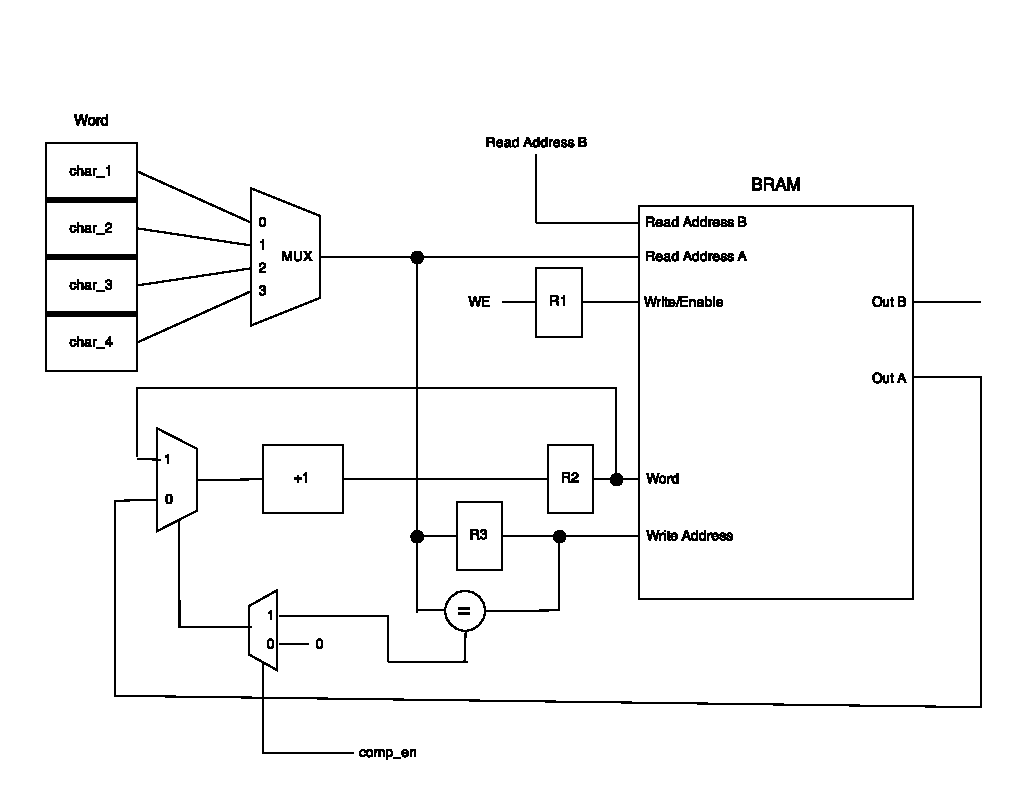
\includegraphics[width=1.0\textwidth]{img/hw_datapath}
    \caption{Datapath do acelerador}
    \label{fig:hw_datapath}
  \end{figure}

  \paragraph{} A \autoref{fig:hw_datapath} mostra a datapath usada no acelerador. Esta recebe 4 caracteres porque cada caracter são 8 bits e a \texttt{FSL} transporta 32 bits. O próprio caracter endereça a \texttt{BRAM}, o valor lido é incrementado e de seguida é guardado na \texttt{BRAM}. Caso exista dois caracters repetidos na palavra em vez de ser incrementado o valor da \texttt{BRAM} é incrementado o valor da contagem calculado anteriormente.

\subsection{Máquina de Estados}
  \begin{figure}[H]
    \centering
    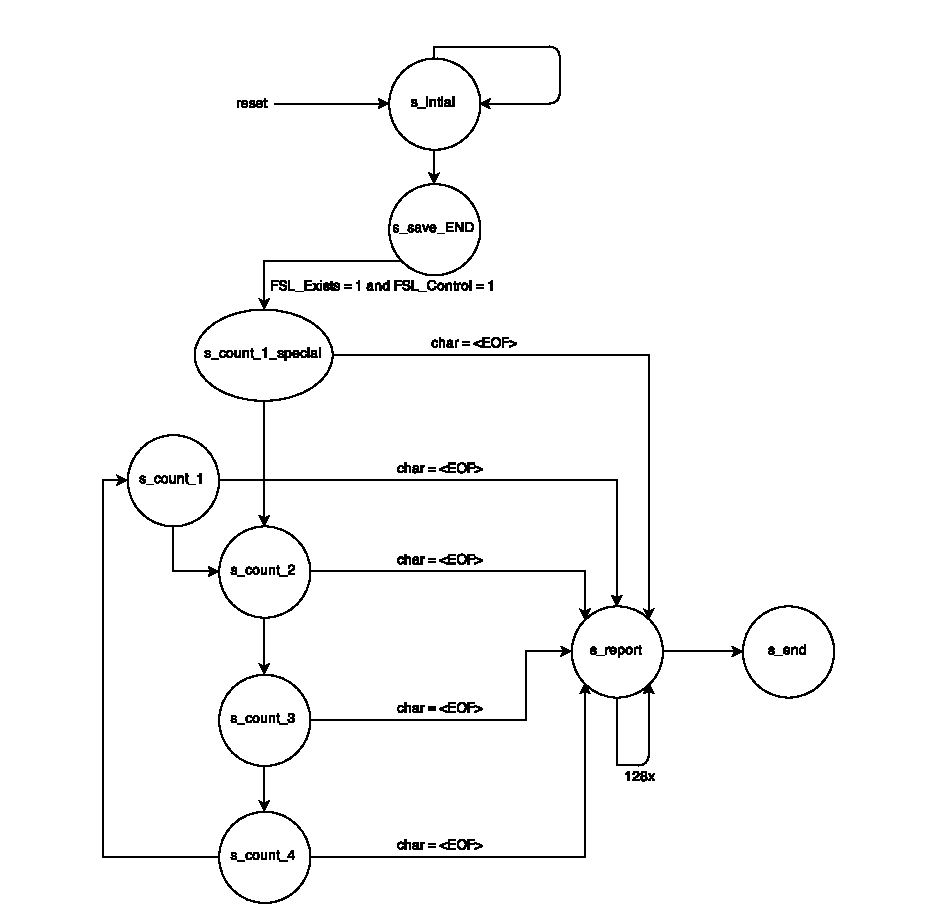
\includegraphics[width=1.0\textwidth]{img/fsm}
    \caption{Máquina de Estados do acelerador}
    \label{fig:hw_fsm}
  \end{figure}

  \paragraph{} A máquina de estados apresentada na \autoref{fig:hw_fsm} é iniciada com o sinal \texttt{FSL\_Reset} e fica presa no estado \texttt{s\_initial} até dados se encontrarem na \texttt{FSL} e ter recebido o caracter terminador (\texttt{<EOF>}). Este é enviado em simultâneo com o sinal de controlo.

  O primeiro estado de contagem, \texttt{s\_count\_1\_special}, é especial pois não tem nenhum caracter anterior com que comparar. Os restantes estados têm que comparar com o caracter anterior e geram a palavra de selector do \texttt{MUX} conforme o caracter que pretendem ler.

  Quando o caracter terminador é encontrado o próximo estado vai ser o \texttt{s\_report}. Neste estado é escrito o conteúdo total da \texttt{BRAM} para o \texttt{FSL}, como cada contagem são 16 bits é possível escrever 2 contagens em simultâneo, repetindo-se 128 vezes.
